\chapter{Theoretical Background: Theorema and Software Engineering, and the Project-Perspective on Programming Paradigms in Wolfram Language}
\label{cha:Theory}

This thesis already started off with rewriting-theory, so in this chapter I would like to focus the relevant insights from Theorema itself, as well as WL-systems-building and WL-paradigms, on practically relevant takeaways for the project part.

\section{Theorema} \label{tma}

Theorema is currently available in Version 2.0, under GPL \cite{noauthor_httpswww3riscjkuatresearchtheoremasoftware_nodate} and inlcuding the full source code on GitHub \cite{noauthor_github_nodate}. A tutorial is available as well. \cite{windsteiger_theorema_2017}

Relating the original goal of The Theorema Project with the current project, this foreword excerpt contextualizes Theorema in the world of theorem provers (as of 2006) by comparing the system to 16 others in the same class of system:

\begin{displayquote}
We can also see clearly from the examples in this collection that the notations
for input and output have to be made more human readable. Several systems do
generate LaTeX output for the discovered proofs, but perhaps additional thought
about formatting output might be valuable. The Theorema Project (system 12
in the present list) made readability of proofs a prime requirement, and their
report shows their success. However, the objective Prof. Bruno Buchberger set
originally for the project was to produce a tool for pedagogic use, not research.
\cite[p. 4]{g_mayrhofer_s_saminger__w_winsteiger_theorema_nodate}
\end{displayquote}

\subsection{Theorema vs Mathematica}

Just as we were interested in disambiguating Mathematica and Wolfram Language, to differentiate Theorema (Language) from the former two:

\begin{displayquote}
All Theorema ‘reasoners’ (provers, solvers, and simplifiers) are written in the programming language of Mathematica. Theorema does not use the Mathematica algorithm library or any implicit mathematical knowledge presupposed in Mathematica algorithms.
\cite[p. 110]{g_mayrhofer_s_saminger__w_winsteiger_theorema_nodate}
\end{displayquote}

In current speak, Theorema is implemented in Wolfram Language - but not using in-built algorithms or knowledge, such as the native experimental (in Version 14.0) functions \( ProofObject \) \cite{noauthor_proofobjectwolfram_nodate} and \( FindEquationalProof \) \cite{noauthor_findequationalproofwolfram_nodate}.

\subsection{\textit{Theorema 2.0} - Theorema Commander, Current Project Structure}

Theorema 2.0 most prominently introduces an interactive graphical user interface (GUI) to realize a full fledged mathematical assistant system, depicted in Figures \ref{fig:splash} (splash screen at application start), \ref{fig:start} (start screen under Windows) and \ref{fig:virtual-keyboard} (again the Theorema Commander, this time under Linux, taken from \cite{windsteiger_theorema_2013}), profiting from GUI-friendly dynamic expressions \cite[p. 76]{noauthor_introduction_nodate} and cascading stylesheets \cite{noauthor_stylesheetswolfram_nodate} both introduced with Mathematica Version 6 to realize a native implementation. The mode of interacting with the system fundamentally changes to be more newcomer friendly, because less relient on prior knowledge of the language:

\begin{figure}[h]
    \centering
    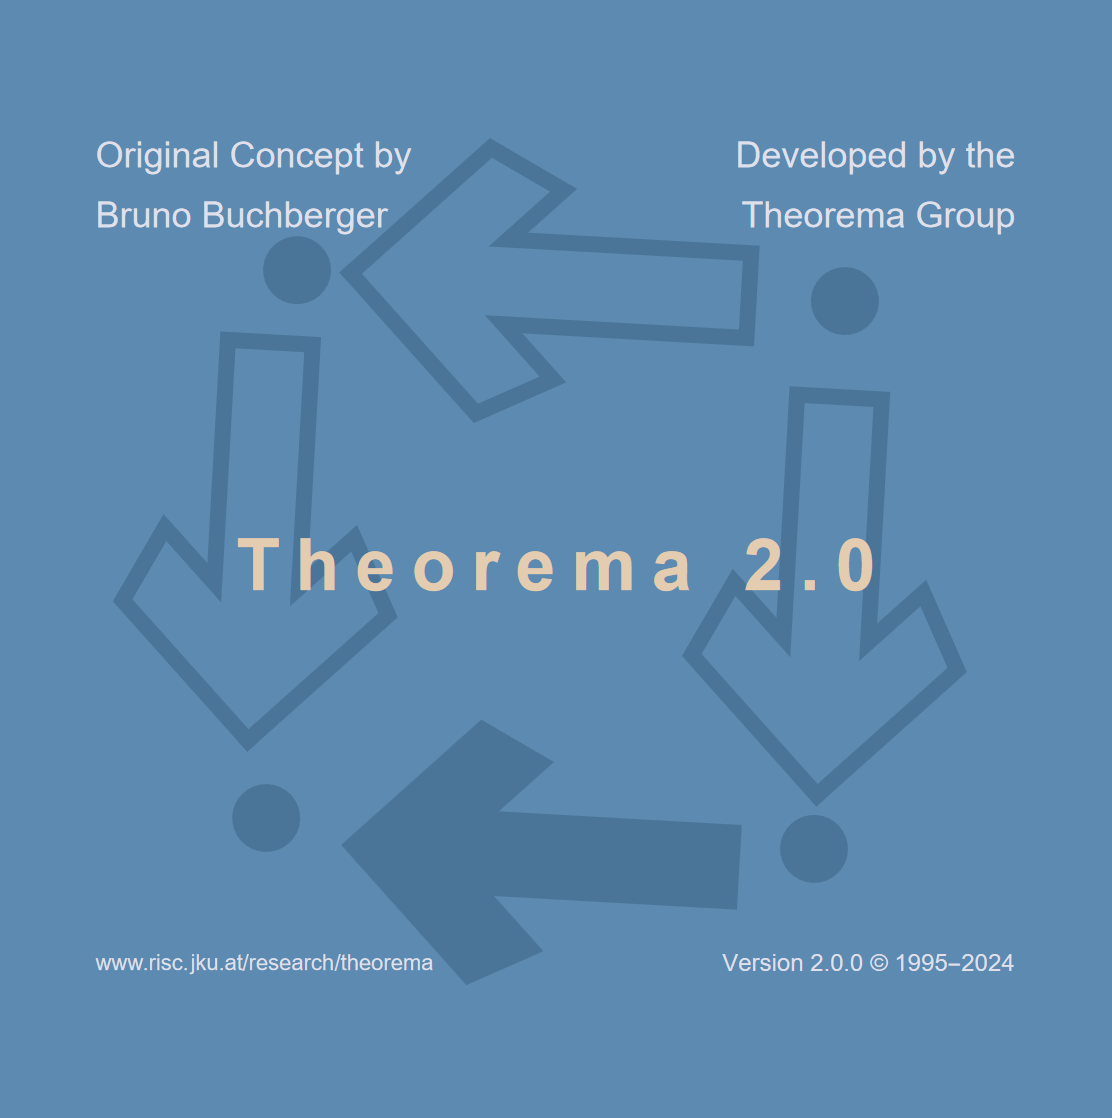
\includegraphics[scale=0.5]{images/theory/splash.png}
    \caption{The Theorema splash screen introducing the project and including a spinning RISC logo in the background.}
    \label{fig:splash}
\end{figure}

\begin{figure}[h]
    \centering
    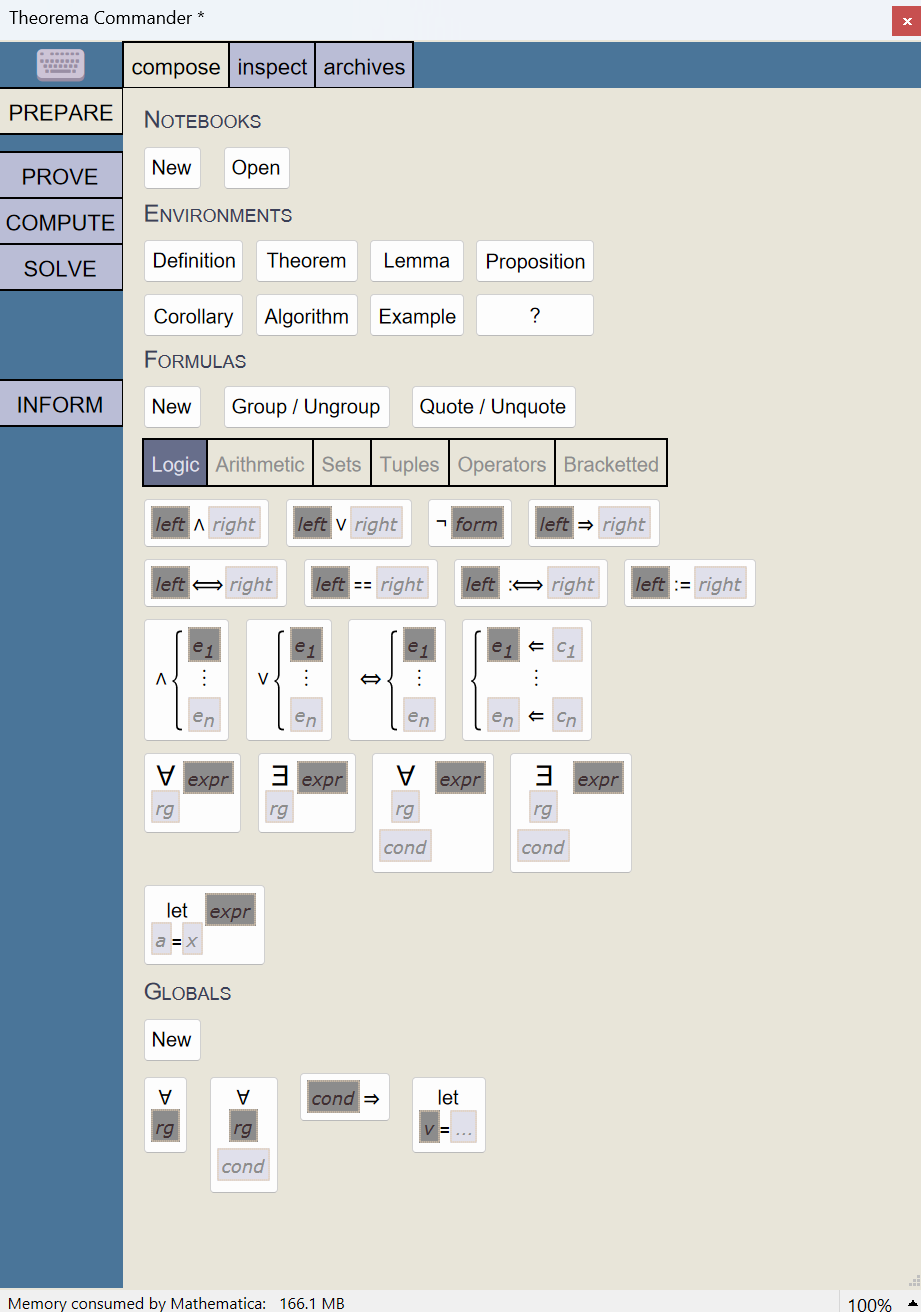
\includegraphics[scale=0.5]{images/theory/start.png}
    \caption{The start view in the Theorema Commander window: on Windows, the Commander opens in its own window, emulating an interface for a separate notebook.}
    \label{fig:start}
\end{figure}

\begin{figure}[h]
    \centering
    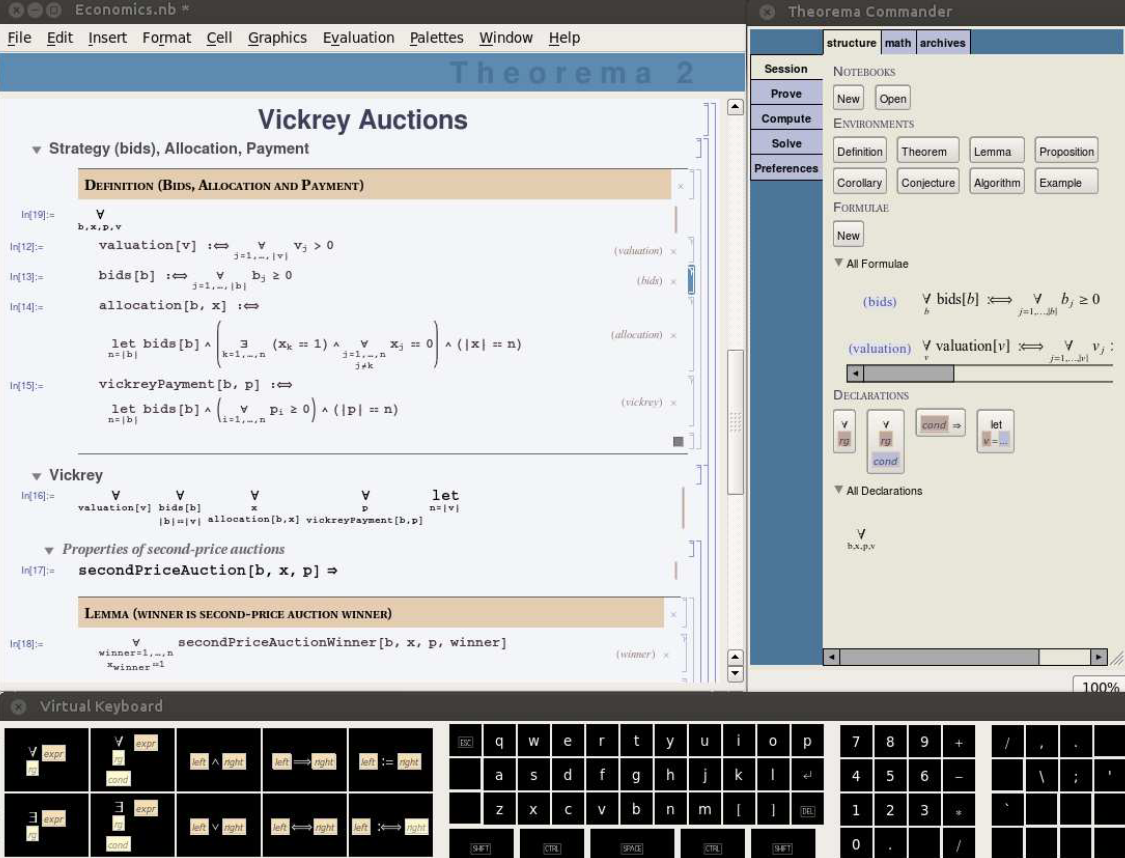
\includegraphics[scale=0.5]{images/theory/virtual-keyboard-linux.png}
    \caption{Taken from \cite{windsteiger_theorema_2013}, this side-by-side view of a notebook with the Commander also shows off the virtual keyboard, including "keys" for formula elements: comparing to the current version of the Commander in \ref{fig:start}, some changes have been made to the interface options, e.g. "Session" appears to be "Prepare"}
    \label{fig:virtual-keyboard}
\end{figure}

\begin{displayquote}
As an example, giving a definition meant evaluation of a \lstinline+Definition[...]+-command, stating a theorem meant evaluation of a \lstinline+Theorem[...]+-command, proving a theorem meant evaluation of a \lstinline+Prove[...]+-command, and performing a computation meant evaluation of a \lstinline+Compute[...]+-command. For the new Theorema 2.0 system, we envisage a more ‘point-and-click’-like interface as one is used to from modern software tools like a mail user agent or office software.
\cite[p. 73]{windsteiger_theorema_2013}
\end{displayquote}

The target user groups are mathematicians and students of mathematics \cite[p. 73]{windsteiger_theorema_2013} Since the Theorema provers are composed of smaller "special prover models" that can be recombined: "In the current status, the access to special prover modules is restricted to the system developers, but a mechanism for users to compose their own provers from available special prover modules is planned for future versions of the system." \cite[p. 111]{g_mayrhofer_s_saminger__w_winsteiger_theorema_nodate}

The current project structure is also made explicit in Figure \ref{tma-dir-tree}.

\subsection{The Logic of Theorema}

'The logic frame of Theorema is higher order
predicate logic, which is extended by the language construct “sequence variables,”' \cite[p. 110]{g_mayrhofer_s_saminger__w_winsteiger_theorema_nodate} already introduced in Section \ref{rewriting} and allowing for pattern matching capabilities. In this view, "the Theorema system is a (growing) collection of various general purpose and special theorem provers. The general purpose provers (like the first order predicate logic natural deduction prover) are valid only for special fragments of predicate logic (e.g. first order predicate logic)." \cite[p. 110]{g_mayrhofer_s_saminger__w_winsteiger_theorema_nodate} The more assumptions are made, the more specialized the prover module that is consulted.

The consequence of this theory for the current project of transforming Theorema documents is that the \LaTeX transformation target language needs to be able to represent Predicate Logic, and particularly, First Order Predicate Logic (FOPL).

\subsection{Theorema Environment and Surfacing the Theorema Language}

Theorema data is read from Mathematica notebooks \cite[p. 75]{windsteiger_theorema_2013}, but exists beyond the data directly visible in the front-end (this needs to be loaded at the appropriate time ahead of the \LaTeX-transformation, so that this authoritative form of the formula is the source of the transformation) - for display purposes, Theorema also defines specific stylesheets, changing the visual appearance from standard Mathematica notebooks, visible in Figure \ref{fig:virtual-keyboard}.

\begin{displayquote}
As soon as the [Theorema] formula is passed to the system through Mathematica’s standard Shift-Enter, the formula is stored in an internal datastructure that carries a unique key for each formula in addition to the formula itself and its label. This key consists of the absolute pathname of the notebook file in which it was given, and the unique cell-ID within that notebook, which is provided by the Mathematica front-end.
\cite[p. 75]{windsteiger_theorema_2013}
\end{displayquote}

We already saw a Theorema formula expression in the introductory chapter \ref{cha:Introduction}, Section \ref{tmaFormulaExpressionExample}: the structure starts like \lstinline+{Theorema`Common`FML$[{"ID:169304498", ...+ where we actually looking at a list of (denoted by curly braces) containing multiple \lstinline+Theorema`Common`FML$+ expressions, each in turn containing a list, and then some more data, but inside the list the first element is the unique cell-ID that the front-end provided. But, "the user never sees nor needs the concrete formula key explicitly." \cite[p. 75]{windsteiger_theorema_2013}

There is a hidden complication at this connection between front-end and internal datastructure: To capture the idea of a scope to make definitions in, Theorema allows for \textit{global declarations}, 'which may either contain one or several "orphaned" universal quantifiers (each containing a variable and an optional condition, but missing the formula, to which thery refer) or an "orphaned" implication (missing the right hand side), or an abbreviation indicated by a "let."' \cite{windsteiger_theorema_2013} names this biimplication:

\begin{center}
   \begin{displayquote}
    bids[\textit{b}] :\Longleftrightarrow \forall_{j=1,\cdots,|\textit{b}|} \textit{b}_j \geq 0
    \cite[p. 76]{windsteiger_theorema_2013}
    \end{displayquote} 
\end{center}

This actually translates to:

\begin{center}
    \begin{displayquote}
    \forall_\textit{b} bids[\textit{b}] :\Longleftrightarrow \forall_{j=1,\cdots,|\textit{b}|} \textit{b}_j \geq 0
    \cite[p. 76]{windsteiger_theorema_2013}
    \end{displayquote}
\end{center}

To make the idea specific to WL, an example from this project's main test notebook, FirstTour.nb, tracing such a declaration from its display in the front-end \ref{fig:global-decl}, to its notebook cell structure \ref{tmaGlobalDeclNotebookCell}, and finally, to its Theorema formula correlate \ref{tmaGlobalDeclFormula}, helps clarify this aspect of Theorema, relevant to the current goal of rendering an accurate output in \LaTeX: The question for the implementation will be how to obtain the Theorema-formula per relevant notebook cell and decide about a full length output (with global declarations) or a somehow trimmed version that is closer to the localized definition: further, it will likely be this hidden Theorema-representation we want to make visible by outputting the output document, rather than the purely-Wolfram-Language representation of the cell (structure) that holds the code for the display of the formula.

\begin{figure}[h]
    \centering
    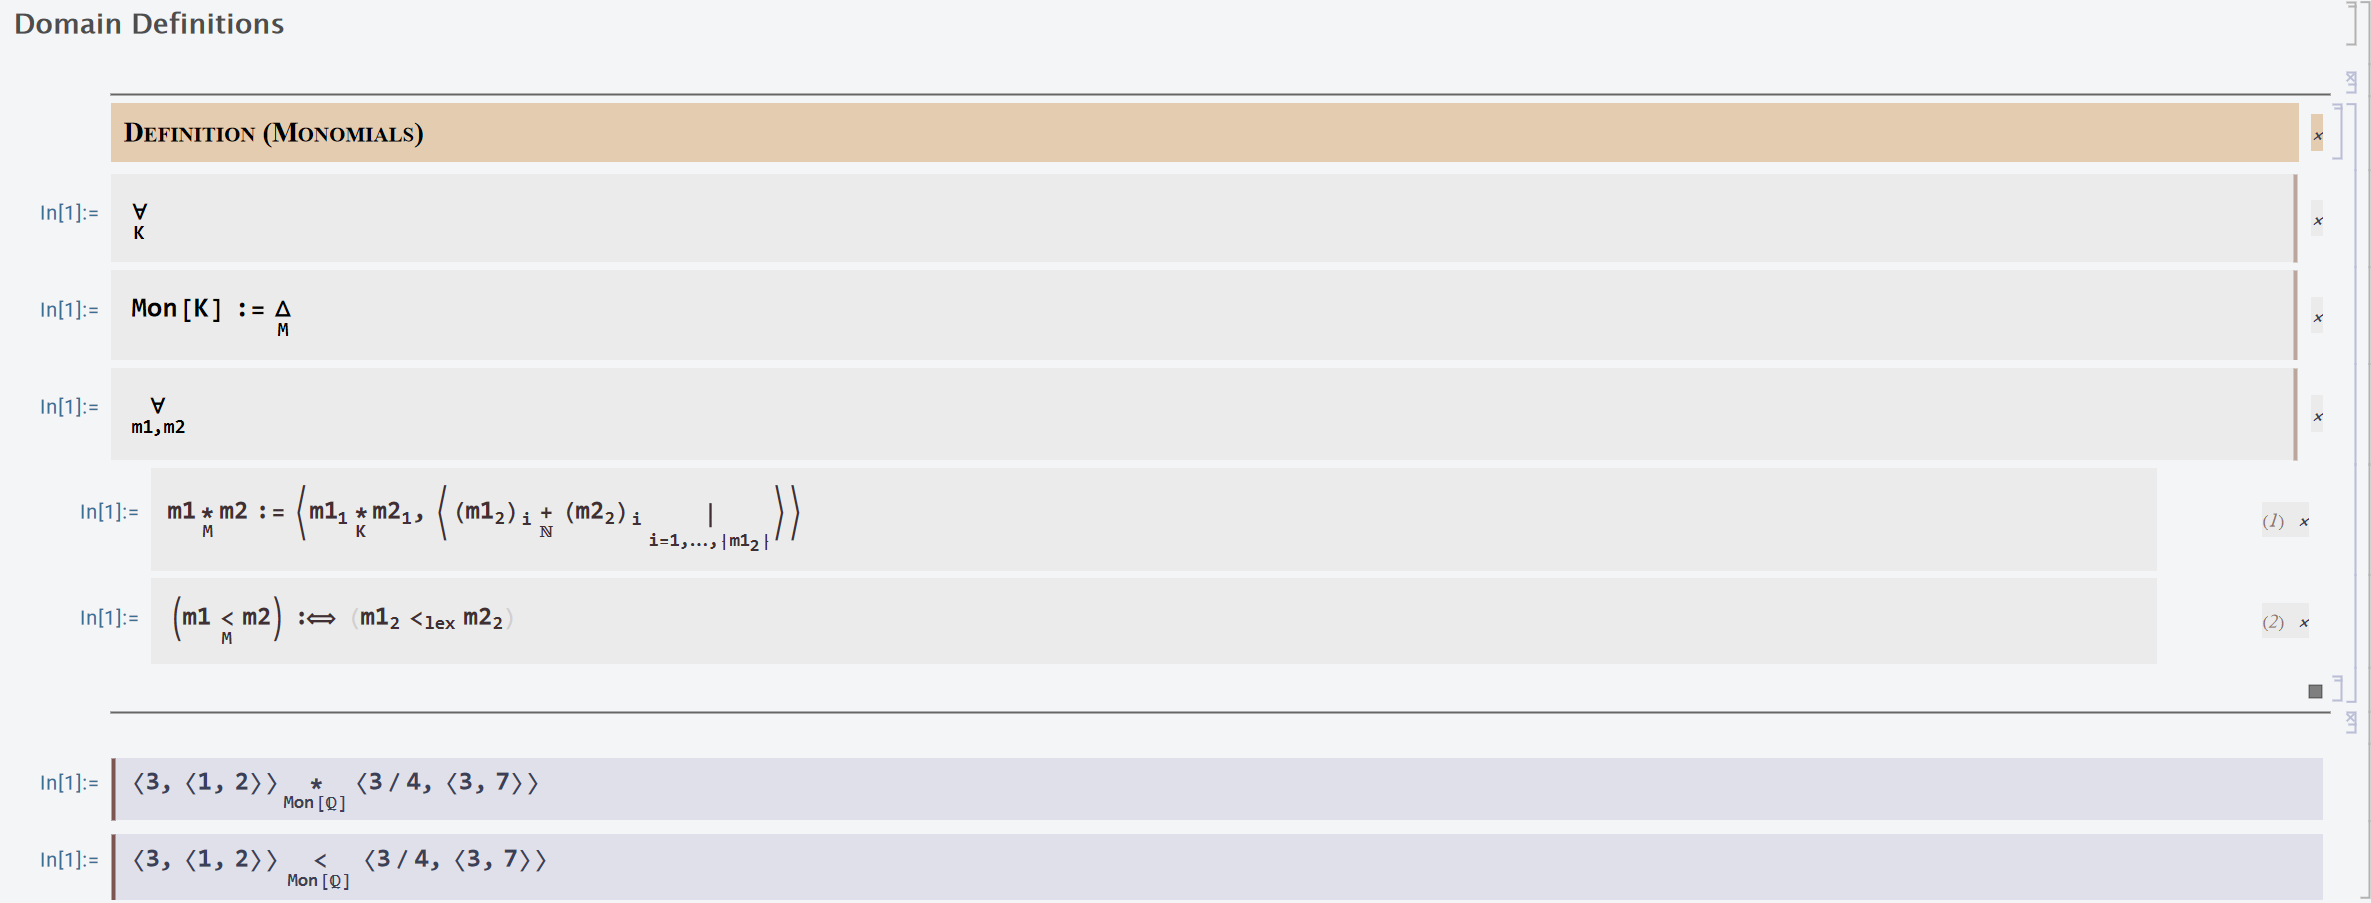
\includegraphics[scale=0.2]{images/theory/global-decl.png}
    \caption{A global declaration in Theorema with three different terms.}
    \label{fig:global-decl}
\end{figure}

\begin{program}
\caption{This is an excerpt from the notebook cell expression depicted in the front-end rendering in Figure \ref{fig:global-decl} and contains just one such global declaration, \lstinline+UnderscriptBox["\[ForAll]", "K"]]+ as the pertinent line from this cell structure.}
\label{tmaGlobalDeclNotebookCell}
\begin{LaTeXCode}
...
Cell[BoxData[
 UnderscriptBox["\[ForAll]", "K"]], "GlobalDeclaration",
 CellFrameLabels->{{None,
    Cell[
     BoxData[
      ButtonBox[
      "\[Times]", Evaluator -> Automatic, Appearance -> None, ButtonFunction :>
       Theorema`Language`Session`Private`removeGlobal[{
         "C:\\Users\\jackh\\OneDrive\\Documents\\RISC2023\\prototype-wolfram-\
lang\\FirstTour.nb", 2090454223}]]]]}, {None, None}},
 ShowCellTags->False,
 CellChangeTimes->{{3.62218621587292*^9, 3.622186218593838*^9}},
 EmphasizeSyntaxErrors->True,
 CellTags->"ID:2090454223",
 CellLabel->"In[1]:=",
 CellID->2090454223,ExpressionUUID->"809f4e1b-f26c-4265-a5d0-d66f43b5b903"]
...
\end{LaTeXCode}
\end{program}

\begin{program}
\caption{This is another Theorema formula and contains as part of it the global declaration term encoded in the notebook expression in \ref{tmaGlobalDeclNotebookCell}.}
\label{tmaGlobalDeclFormula}
\begin{LaTeXCode}
Theorema`Common`FML$[{"ID:2008910260", 
  "Source:C:\\Users\\jackh\\git\\repository\\tma2tex\\FirstTour.nb"}, 
 Theorema`Language`EqualDef$TM[
  Theorema`Language`DomainOperation$TM[Theorema`Knowledge`M$TM, 
    Theorema`Language`Times$TM][Theorema`Knowledge`m1$TM, 
   Theorema`Knowledge`m2$TM], 
  Theorema`Language`Tuple$TM[
   Theorema`Language`DomainOperation$TM[Theorema`Language`K$TM, 
     Theorema`Language`Times$TM][
    Theorema`Language`Subscript$TM[Theorema`Knowledge`m1$TM, 1], 
    Theorema`Language`Subscript$TM[Theorema`Knowledge`m2$TM, 1]], 
   Theorema`Language`TupleOf$TM[
    Theorema`Language`RNG$[
     Theorema`Language`STEPRNG$[
      Theorema`Language`VAR$[Theorema`Knowledge`VAR$i$TM], 1, 
      Theorema`Language`BracketingBar$TM[
       Theorema`Language`Subscript$TM[Theorema`Knowledge`m1$TM, 2]], 
      1]], True, 
    Theorema`Language`DomainOperation$TM[
      Theorema`Language`IntegerInterval$TM[1, \[Infinity], True, 
       False], Theorema`Language`Plus$TM][
     Theorema`Language`Subscript$TM[
      Theorema`Language`Subscript$TM[Theorema`Knowledge`m1$TM, 2], 
      Theorema`Language`VAR$[Theorema`Knowledge`VAR$i$TM]], 
     Theorema`Language`Subscript$TM[
      Theorema`Language`Subscript$TM[Theorema`Knowledge`m2$TM, 2], 
      Theorema`Language`VAR$[Theorema`Knowledge`VAR$i$TM]]]]]], "1"]
\end{LaTeXCode}
\end{program}

\section{Large Systems with Wolfram Language} \label{large-sytems}

Wolfram Research advocates for building large systems in WL and cites the WL system itself as "one of the more complex software systems ever constructed. It is built from several million lines of source code, written in C/C++, Java, and the Wolfram Language." \cite[The Software Engineering of the Wolfram System]{noauthor_internals_nodate} Wolfram Research cites the following general principles and more as they concern building large systems in any language \cite{noauthor_building_nodate}:

\begin{itemize}
    \item Divide the System into Components
    \item Write and Use Unit Tests
    \item Think of the Architecture, Not the Code
    \item Use Source Control
    \item Write Documentation
\end{itemize}

There are also WL-specific advantages in Software Engineering, explored in \cite[Take Advantage of the Wolfram Language]{noauthor_building_nodate}.

\subsection{Modularity with Packages} \label{modularity}

In WL, Package development \cite{noauthor_package_nodate}, namespace management \cite{noauthor_namespace_nodate}, and further scoping constructs \cite{noauthor_scoping_nodate} are interrelated and form the extensibility of the system: A typical Wolfram Language package is a .wl or .m file that contains a collection of functions and variables. These packages are structured in a way that separates the implementation from the interface, often using \lstinline+BeginPackage[]+ \cite{noauthor_endpackagewolfram_nodate} and \lstinline+EndPackage[]+ \cite{noauthor_endpackagewolfram_nodate} to define the public interface and \lstinline+Begin[]+ \cite{noauthor_beginwolfram_nodate} and \lstinline+End[]+ \cite{noauthor_endwolfram_nodate} for the implementation section.

Contexts are used to manage namespaces \cite{noauthor_namespace_nodate} , preventing name collisions between different packages or within different parts of the same package. By convention, package names serve as contexts, which helps in organizing the functions and variables and avoiding naming conflicts. Packages in the Wolfram Language use \lstinline+Get[]+ (\lstinline+<<+) \cite{noauthor_getwolfram_nodate} for loading, which executes the package code, effectively defining the functions and variables in the specified context. (\lstinline+Needs[]+ is the alternative, only loading loading the package if the specified context is not already in \lstinline+$Packages+, the relevant context variable in this case. \cite{noauthor_needswolfram_nodate})

\subsection{Theorema as an Extensible Mathematica Package} \label{extensible-package}

Theorema can be loaded like any WL-package but is really a collection of Wolfram Language packages, see \ref{tma-dir-tree} - the proposed format of the functionality implemented with this project is therefore also a WL-package, a file with file ending ".wl" (current) or ".m" (historically) and following the layout given by this Theorema template file ("Theorema
/PackageTemplate.m" \cite{noauthor_theorematheoremapackagetemplatem_nodate}) - including the copyright statement, which bakes the GNU (a recursive acronym, ""GNU's Not Unix:" The GNU Project was initiated by Richard Stallman in 1983 and is a free software, mass collaboration project \cite{noauthor_gnu_nodate-1}) licensing in right at the point of extensibility and states that anyone is free to redistribute and/or modify the software under the terms of the GPL (General Public License). \cite{noauthor_gnu_nodate} (However, the software is provided without any warranty.)

\begin{figure}[ht]
\centering
\vspace{10pt} % Adds 10 points of vertical space. Adjust the value as needed.
\begin{forest}
  for tree={
    font=\ttfamily,
    grow'=0,
    child anchor=west,
    parent anchor=south,
    anchor=west,
    calign=first,
    edge path={
      \noexpand\path [draw, \forestoption{edge}]
      (!u.south west) +(7.5pt,0) |- (.child anchor) \forestoption{edge label};
    },
    before typesetting nodes={
      if n=1
        {insert before={[,phantom]}}
        {}
    },
    fit=band,
    before computing xy={l=15pt},
  }
[Theorema
  [Computation]
  [Documentation
    [English]
  ]
  [FrontEnd]
  [Interface]
  [Kernel]
  [Knowledge]
  [Language]
  [Provers]
  [System]
]
\end{forest}
\caption{Directory Structure of the main directory in the Theorema project; directories are filled with .m-Mathematica/WL package files.}
\label{tma-dir-tree}
\end{figure}


\section{Paradigms: The Project-Perspective on the Multi-Paradigm Approach in Wolfram Language}

WL supports multiple programming paradigms, including the procedural one: "The Wolfram Language supports all standard procedural programming constructs, but often extends them through integration into its more general symbolic programming environment." \cite{noauthor_procedural_nodate} While not a pure OOP (Object Oriented Programming) language, WL can mimic OOP concepts through associative arrays (Associations) and symbolic structures, as outlined in Section \ref{oop}. 

\subsection{Functional vs Procedural Programming in Wolfram Language, and the High-Level Programming Paradigm} \label{high-level}

Functional programming in WL is introduced in the Wolfram Research documentation center as well \cite{noauthor_functional_nodate}, and exploring this in the context of high level programming is particularly fruitful, since the the combination of abstracted functionality with functional approaches can make for readable code. The present author would like to reference his exposé \ref{app:Expose} of the topic of contrasting these programming styles as they are applied to one particular example, Program \ref{treeProgram} and move on to the rule-based approach most relevant for the project at hand, after citing the seamless conversion of geometric objects to Unity (the game engine \cite{noauthor_real-time_nodate}) objects just one example of the high-level, abstracted idea of providing functionality in the WL ecosystem: 

\begin{center}
   \begin{displayquote}
    Drawing on its algorithmic power, Version 12 provides high–level functions that are uniquely easy to use to create and manipulate Unity objects. Easily create game objects with \lstinline+CreateUnityGameObject+ and directly include geospatial and socioeconomic data, and across thousands of domains.
    \cite{noauthor_highlevel_nodate}
    \end{displayquote} 
\end{center}

\begin{figure}[h]
    \centering
    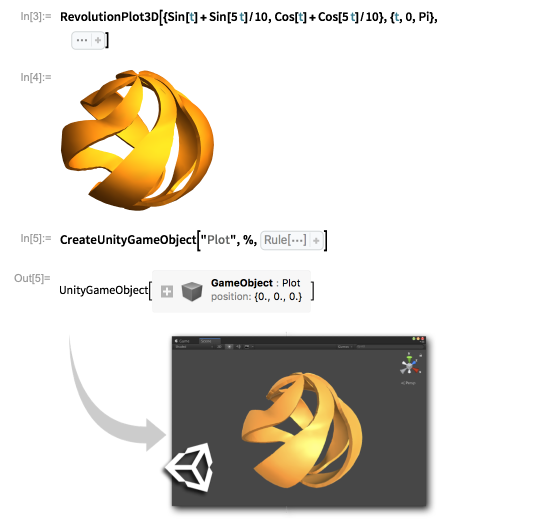
\includegraphics[scale=0.5]{images/theory/unity.png}
    \caption{Plots, graphics, and geometric objects are automatically converted to Unity's mesh format during the creation of a game object.\cite{noauthor_highlevel_nodate}}
    \label{fig:unity}
\end{figure}

Curated knowledge (data packages) available directly inside the WL system complement this paradigm-combination, as is made apparent in this example - see also Figure \ref{fig:unity}.

\begin{program}
\caption{These functions extract a tree data structure in the form of certain integer mathematical proof IDs and the related children IDs from a grid expression in WL and serve well to illustrate lists and replacements, functional and rule-based programming, as well as recursion, for efficient implementations. An expose with details is part of the appendix in the present work. \ref{app:Expose}}
\label{treeProgram}
\begin{LaTeXCode}
proofID[Grid[{___,{ID,id_},___},___]]:=id;
subproofs[
Grid[{___, {Proofs, OpenerView[{Arguments, Column[subproofs_, ___]}, ___]}, ___},
___]] := subproofs; subproofs[proof_] := {};
getLeanTree[proof_] := Tree[proofID[proof], getLeanTree /@ subproofs[proof], TreeElementLabelStyle  All  Directive[White, 16, FontFamily  "Times New Roman"], TreeElementStyle  All  Directive[EdgeForm[Black], RGBColor["#B6094A"]]]
\end{LaTeXCode}
\end{program}

\subsection{Symbolic Expressions Lead to Rule-Based Programming and Pattern Matching Approaches} \label{symbolic-expressions}

\subsection{Rule-Based Programming}

Another prominent mathematical research institute in Linz works with Mathematica \cite{noauthor_institute_nodate}, extending its rule-based programming capacity in the $\rho$Log package \cite{marin_rule-based_nodate} - much like Buchberger, Marin and Piroi identify Mathematica as a powerful system implementing the paradigm they are interested in, rule-based programming, the more general one as compared to (term) rewriting: While both concepts rely on rules, term rewriting is a specific type of rule-based operation focused on the transformation of expressions, whereas rule-based programming is a broader paradigm that can dictate various aspects of a program's behavior based on predefined logical rules.

This project's goals make the rule-based programming paradigm clearer. The author's outline the features lacking in Mathematica in terms of rule-based programming:

\begin{center}
    \begin{displayquote}
    \begin{enumerate}
        \item The possibility to program compositions of reductions, alternative choices, reflexive-transitive closures, etc.
        \item A built-in search mechanism to decide the existence of derivations $\text{Expr}_1$ $\rightarrow_{rr}$ $\text{Expr}_2$, where $\text{Expr}_1$, $\text{Expr}_2$ are given expression schemata (patterns), and $\rightarrow_{rr}$ is a specification of a sequence of rule reduction steps. Typically, the specification of $\rightarrow_{rr}$ is built with the operators mentioned before (composition, choices, etc.)
        \item The possibility to generate proofs which justify the existence or non-existence of such reduction derivations.
    \end{enumerate}
        \cite{marin_rule-based_nodate}
    \end{displayquote} 
\end{center}

To address these shortcomings, they simply implement a package to extend Mathematica according to their needs, achieving the following and demonstrating the flexibility of the system in this way.

\begin{center}
    \begin{displayquote}
    \begin{enumerate}
        \item Concise means to express the basic computational steps of an intended rule application as basic rules. These features are inherited from Mathematica, whose computational engine is based on a higher-order rewrite logic and with advanced support for symbolic and numeric computing.
        \item Programming constructs, such as conditional basic rules and rule combinators, which make it possible to structure large specifications of rules.
        \item Built-in search mechanism to answer queries of the form $\exists\{R_1,...,R_k\} \text{Expr}_1 \rightarrow_r \text{Expr}_2$ where $\text{Expr}_1$ is a ground expression, $r$ is the identifier of a rule, and $\text{Expr}_2$ is a Mathematica pattern whose variables are named $R_1, \ldots, R_k$ (see Section 2.2) [of \cite{marin_rule-based_nodate}].
        \item Support for generating proof objects, i.e., certificates that justify the correctness of the answer provided by $\rho$Log to a query.
        \item Visualization tools for proof objects, which enable the analysis of the deduction derivations of $\rho$Log in a natural language formulation and at various levels of detail.
    \end{enumerate}
        \cite{marin_rule-based_nodate}
    \end{displayquote} 
\end{center}

In both contexts, symbolic expressions are not just passive data; they are actively transformed or evaluated as part of the computational process. These expressions provide a versatile and powerful means to represent and manipulate knowledge, logic, and computations in a way that is abstracted from the specific details of the underlying data, allowing for more generalized and flexible rule application and system behavior.

\subsection{Rule-Based Programming vs Rewriting, via Pattern Matching}
\label{sec:rule_vs_rewriting}

Rule-based programming focuses on defining rules that guide the transformation of expressions within a program. It is declarative, meaning it specifies \textit{what} should be done rather than \textit{how} to do it. Rules are applied to expressions iteratively until no further rules can be applied or until a certain condition is met.

Pattern matching is a technique often used within rule-based programming but is more specifically focused on identifying parts of an expression that match a certain form. Pattern matching is integral to the process of identifying where and how rules should be applied in rule-based programming. Not all pattern matching is necessarily linked to rule-based programming.

Rewriting, while similar to rule-based programming, is a specific subset focused on the transformation of expressions through specific rules. It operates under the paradigm of applying these rules to achieve a specific form or outcome. Rewriting is a more specialized operation compared to the broader scope of rule-based programming.

\subsubsection*{Key Differences}
\begin{itemize}
    \item \textbf{Scope:} Rule-based programming can encompass various aspects of program behavior dictated by rules, whereas rewriting is a particular technique within this broader paradigm.
    \item \textbf{Focus:} Rule-based programming is concerned with defining transformations (the \textit{what}), while pattern matching focuses on identifying parts of an expression that need transformation (the \textit{identification}).
    \item \textbf{Application:} Pattern matching serves the rule-based programming paradigm by identifying where rules apply, while rule-based programming defines what transformations to apply.
\end{itemize}

\subsubsection*{Integration}
In the context of Wolfram Language and systems like Theorema, rule-based programming and pattern matching are core tools used to process and transform symbolic expressions. The interplay of these techniques allows for flexible and powerful manipulation of expressions, crucial for this project's task of converting mathematical expressions into \LaTeX.
